\subsubsection{Fit}

Eseguiamo il fit ai minimi quadrati del rate in funzione dell'angolo,
assegnando l'incertezza poissoniana ai rate e \SI{\pm1}{\degree} agli angoli.
Nel caso di collimatore da \SI1{mm} usiamo una funzione proporzionale alla \eqref{eq:rutherford}:
\begin{align}
	\label{eq:fit1}
	R_1(\theta;B,\theta_0)
	&= \frac {B} {(1-\cos(y(\theta-\theta_0)))^2}, \\
	y(\theta)
	&= \theta + (\operatorname{sgn} \theta) \theta_\text{min} e^{-|\theta|/\theta_\text{min}},
	\quad \theta_\text{min} = \SI{0.2}{\degree}, \notag
\end{align}
dove $y$ serve solo a regolarizzare la funzione per il conto numerico ($\theta_\text{min}$ non influisce sul fit).
Per il collimatore da \SI5{mm} mediamo la \eqref{eq:fit1}
supponendo che il fascio incidente abbia una distribuzione uniforme sul collimatore:
\begin{align*}
	R_5(\theta;B,\theta_0)
	&= \int_{-\ell/2}^{\ell/2} \frac{\de a}{\ell}
	\frac B {(1-\cos(y(\theta_R(a, \theta-\theta_0))))^2}, \\
	\theta_R(a, \theta)
	&= \tan^{-1} \left( \tan(\theta) - \frac a {L\cos\theta} \right) - \tan^{-1}\frac aD,
\end{align*}
dove $a$ è la coordinata sul collimatore, $\theta_R$ è l'angolo di cui effettivamente viene deviata la traiettoria attraversando il bersaglio,
$L$ e $D$ sono definite in \autoref{sec:forma}, $\ell$ è la larghezza del collimatore.
I dati con sovraimposte le curve di fit sono riportati in \autoref{fig:fit},
i risultati sono riportati in \autoref{tab:fit}.

\begin{figure}
	\hspace{-0.2\textwidth}
	{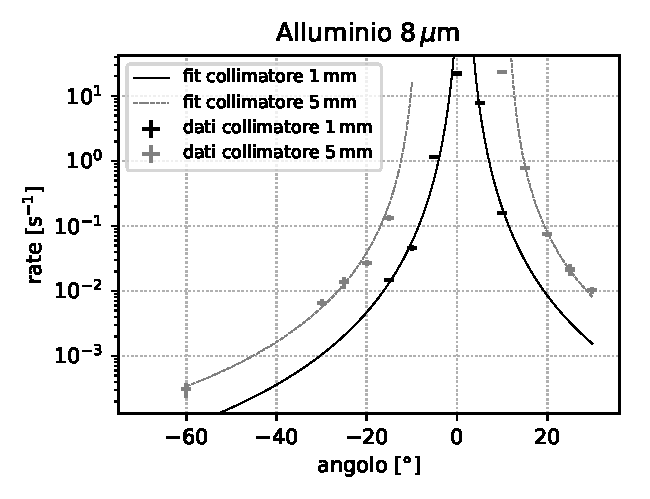
\includegraphics[height=0.5\textwidth]{immagini/all}}
	~
	{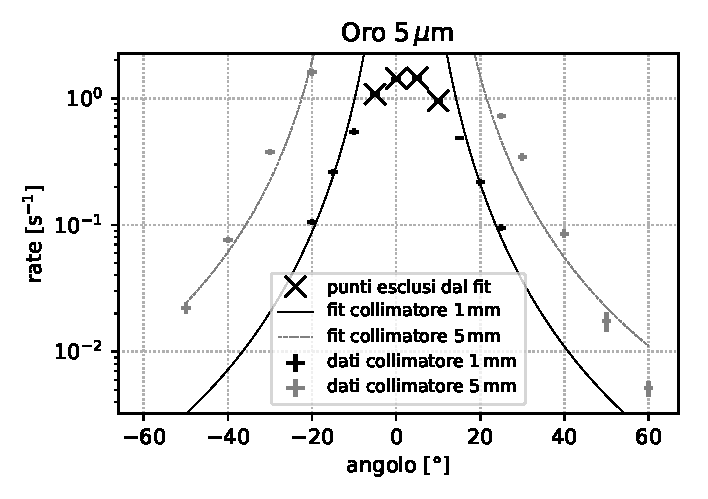
\includegraphics[height=0.5\textwidth]{immagini/oro5}}
	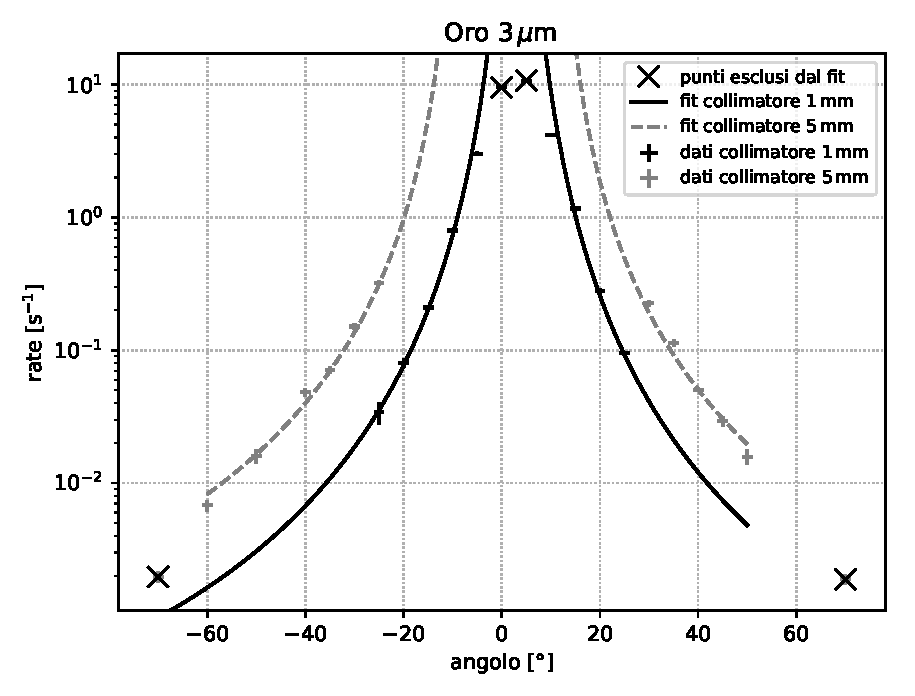
\includegraphics[height=0.5\textwidth]{immagini/oro3}
	\caption{\label{fig:fit}
	Dati e curve di fit.
	Sono esclusi dal fit i punti vicini a \SI0{\degree},
	ma anche i~punti a \SI{\pm70}{\degree} perché hanno un rate troppo minore di quello atteso
	(come anche suggerito dalla simulazione).}
\end{figure}

\begin{table}
	\centering
	\begin{tabular}{cccrrc}
		Bersaglio & $B$ [\si{s^{-1}}] & $\theta_0$ [\si\degree] & corr. & $\chi^2$/dof & $B_5/B_1$ \\
		\hline
		\texttt{al8coll1} & \num{5.7(11)e-6 } & \num{1.5 \pm 0.5  } & \SI{41.5} \% & 3.1 / 4  & \\
		\texttt{al8coll5} & \num{2.19(19)e-5} & \num{1.2 \pm 0.4  } & \SI{8.8 }\%  & 10.7 / 8 & \num{3.9 \pm 0.8} \\
		\texttt{au3coll1} & \num{1.22(10)e-4} & \num{3.02 \pm 0.35} & \SI{9.1 }\%  & 3.8 / 7  & \\
		\texttt{au3coll5} & \num{5.26(22)e-4} & \num{1.1 \pm 0.4  } & \SI{5.8 }\%  & 11.1 / 9 & \num{4.3 \pm 0.4} \\
		\texttt{au5coll1} & \num{1.21(11)e-4} & \num{2.2 \pm 0.4  } & \SI{-1.4} \% & 7.9 / 4  & \\
		\texttt{au5coll5} & \num{6.8(3)e-4  } & \num{-0.5 \pm 0.4 } & \SI{-6.2} \% & 80.5 / 7 & \num{5.6 \pm 0.6} 
	\end{tabular}
	\caption{\label{tab:fit}
	Risultati del fit. Il bersaglio è indicato come
	\texttt{<elemento><spessore [\si{\micro m}]>coll<collimatore [\si{mm}]>}.
	Il rapporto $B_5/B_1$ è il rapporto tra i $B$ con il collimatore da 5 e quello da 1.}
\end{table}

\subsubsection{Rapporto delle cariche nucleari}

Comparando i parametri di ampiezza dei fit con l'oro con quello eseguito sull'alluminio
possiamo estrarre il rapporto delle cariche nucleari.
Le ampiezze di fit hanno la forma
$$ B=\mathcal{L} \left( \frac {zZ\alpha\hbar c} {2T} \right)^2 = \mathcal{L} A. $$
La nostra luminosità vale $\mathcal{L}=r n l$, in cui $r$ è il rate di particelle incidenti, $n$  è la densità di bersagli e $l$ è lo spessore del bersaglio.
Nel nostro caso $r$ è uguale per tutte le misure con lo stesso collimatore.
Allora il rapporto è dato da:
\begin{equation*}
\frac {Z_{\text{Al}}} {Z_{\text{Au}}}
= \sqrt{ \frac{B_{\text{Al}}}{B_{\text{Au}}} \frac{n_{\text{Au}} l_{\text{Au}}}{n_{\text{Al}} l_{\text{Al}}} }.
\end{equation*}
Fissando $Z_\text{Au}=79$ otteniamo i seguenti risultati:
\begin{align*}
\text{Oro } \SI3{\micro m}&:\\
\text{collimatore } \SI1{mm}&: Z_{\text{Al}}=\num{10.4\pm1.1} \\
\text{collimatore } \SI5{mm}&: Z_{\text{Al}}=\num{9.8\pm0.5} \\
\text{Oro } \SI5{\micro m}&:\\           
\text{collimatore } \SI1{mm}&: Z_{\text{Al}}=\num{13.4\pm1.4} \\
\text{collimatore } \SI5{mm}&: Z_{\text{Al}}=\num{11.1\pm0.5} \\
\end{align*}
L'incertezza è solo quella di fit di $B$.
Soltanto le misure con collimatore da \SI{1}{mm} sono compatibili con il valore noto $Z_\text{Al}=13$.
